\documentclass[12pt]{article}
\usepackage[utf8]{inputenc}
\usepackage{amsmath}
\usepackage{graphicx}
\usepackage{float} % For [H] figure placement
\usepackage{caption} % For caption styling
\usepackage{subcaption} % For subfigures
\usepackage{geometry}
\geometry{a4paper, margin=1in}
\usepackage{booktabs} % For professional quality tables
\usepackage{listings} % For embedding code snippets
\usepackage{xcolor}   % For coloring in listings
\usepackage{hyperref}
\hypersetup{
    colorlinks=true,
    linkcolor=black,
    urlcolor=black,
    citecolor=black,
    filecolor=black,
    anchorcolor=black,
    linktocpage=true
}
\usepackage{hypcap} % Should be loaded after hyperref for correct anchor placement


\title{Disease Simulation Project \\ \large CS 1382 - Discrete Computational Structures}
\author{Andres Antillon}
\date{May 9, 2025 \\ \vspace{0.5em} \small Instructor: Dr. Jos\'{e} Carranza-Rojas \\ \small Texas Tech University - Costa Rica \\ \small Spring 2025 Term}

\begin{document}

\maketitle
\tableofcontents
\newpage

\section{Project Overview}
This project, "Disease Simulation," explores discrete computational structures through the modeling of infectious disease spread in a networked population. It implements various infection models and allows for configurable simulations to observe different epidemiological dynamics. The primary focus is on the software design, implementation of probabilistic models, and graph-based interactions, rather than an in-depth epidemiological study. The simulation framework is built in Python, utilizing libraries such as NetworkX for graph manipulation, NumPy for numerical operations, and Matplotlib/Seaborn for plotting results.

\section{Graph Creation and Population Setup}
The foundation of the simulation is a population represented as a network graph, generated by the \texttt{src/graph\_setup.py} module.

\subsection{Graph Generation Models}
The simulation supports three primary graph generation models to represent the population network, configurable via the \texttt{graph\_type} parameter within the JSON configuration files:
\begin{itemize}
    \item \textbf{Erdos-Renyi (Default):} Creates a random graph where each of the $N$ nodes (specified by \texttt{population\_size}) is connected to every other node with a uniform probability $p$ (specified by the \texttt{connections} parameter). This model tends to produce graphs with a Poisson degree distribution.
    \item \textbf{Barabasi-Albert:} Generates a scale-free network using a preferential attachment mechanism. Starting with a small initial set of connected nodes, new nodes are added one by one. Each new node forms $m$ (specified by \texttt{connections}) links to existing nodes, with the probability of connecting to a given existing node being proportional to its current degree. This results in a power-law degree distribution, characteristic of many real-world networks.
    \item \textbf{Watts-Strogatz:} Produces a small-world network, characterized by high clustering and short average path lengths. It begins with a regular ring lattice where each node is connected to its $k$ (specified by \texttt{connections}) nearest neighbors. Then, each edge is rewired with a fixed probability (hardcoded to $p=0.1$ in this implementation) to a randomly chosen node.
\end{itemize}

The logic for selecting and creating the appropriate graph type based on configuration is implemented in \texttt{src/graph\_setup.py}.

\subsection{Node Attribute Sampling}
Node attributes such as \texttt{immune\_level}, \texttt{vaccine\_ef\-fec\-tive\-ness}, and initial infection status are sampled from distributions specified in the configuration. This initialization logic is implemented in \texttt{src/graph\_setup.py}.

\subsection{Edge Attribute Sampling}
Edges can have a \texttt{contact\_chance} attribute, also sampled from a normal distribution as defined in the configuration. This parameter influences the probability of infection transmission along that edge. The edge attribute initialization is handled in \url{src/graph_setup.py}.

\section{Infection Models}
Three distinct infection models are implemented to calculate the daily probability of a susceptible node becoming infected based on its infected neighbors and individual characteristics. Each model represents a different approach to modeling disease transmission dynamics.

\subsection{Independent Infection Model}
The Independent Infection Model is implemented in \texttt{src/models/independent.py}.
\subsubsection{Mechanism}
For each susceptible node, the model calculates the probability of infection from each infected neighbor independently. The probability of infection from a single infected neighbor is based on a base transmission probability adjusted by the susceptible node's immunity level and vaccine effectiveness:
\[ P(\text{infection from one neighbor}) = P_{\text{base}} \times (1 - L_{\text{immune}}) \times (1 - E_{\text{vaccine}}) \]
The overall probability of infection for the susceptible node on a given day is:
\[ P(\text{infection}) = 1 - \prod_{i \in \text{InfectedNeighbors}} (1 - P(\text{infection from neighbor } i)) \]
\subsubsection{Implications}
This model assumes independence between transmission events from different neighbors, reflecting a scenario where each contact with an infected individual carries its own risk, and multiple contacts compound the risk in a straightforward multiplicative manner.

\subsection{Dependent (Sigmoid) Infection Model}
The Dependent Infection Model, also referred to as the Sigmoid model, is implemented in \texttt{src/models/dependent.py}.
\subsubsection{Mechanism}
Unlike the independent model, this approach calculates the probability of infection as a function of the \textit{number} of infected neighbors, $k$, using a sigmoid function:
\[ P_{\text{sigmoid}} = \frac{1}{1 + e^{-\alpha k + \beta}} \]
where $\alpha$ and $\beta$ are parameters controlling the steepness and shift of the sigmoid curve, respectively. This $P_{\text{sigmoid}}$ is then adjusted by the susceptible node's \texttt{immune\_level} and \texttt{vaccine\_ef\-fec\-tive\-ness}:
\[ P(\text{infection}) = P_{\text{sigmoid}} \times (1 - L_{\text{immune}}) \times (1 - E_{\text{vaccine}}) \]
\subsubsection{Implications}
This model captures a threshold effect, where the risk of infection increases sharply once a certain number of infected neighbors is reached, simulating scenarios where social clustering or repeated exposure significantly amplifies risk beyond a linear accumulation.

\subsection{Superspreader Dynamic Infection Model}
The Superspreader Dynamic Infection Model is implemented in \texttt{src/models/super\-spreader.py}.
\subsubsection{Mechanism}
This model builds on the Independent Infection Model but introduces the concept of superspreaders—individuals with significantly higher infectivity. Each infected individual has a daily probability of becoming a superspreader. If designated as a superspreader for that day, their base infectivity is multiplied by a configurable factor, making them more likely to infect their neighbors.
\subsubsection{Implications}
This model reflects scenarios where a small number of individuals can be disproportionately responsible for a large number of transmissions (the 80/20 rule). It introduces significant heterogeneity in infectiousness, both over time for a single individual and across the infected population. This can lead to potentially more explosive, less predictable outbreaks with rapid bursts of infection, compared to models with uniform or more homogeneous infectivity.

\section{Simulation Configuration and Execution}
The simulation process is orchestrated by the \texttt{Simulation} class in \texttt{src/simulation.py} and initiated via \texttt{main.py}. Simulations are configured and driven by JSON files that specify all parameters, from graph type to infection model specifics. These files are typically located in the \texttt{configs/} directory, often organized into experimental suites (e.g., \texttt{configs/exp1\_{}foun\-da\-tions/}). The \texttt{src/config.py} module, particularly its \texttt{load\_config} function, plays a key role in handling these configurations.

The core simulation step involves updating node states based on infection probabilities calculated by the active model, tracking recoveries, and recording statistics for later analysis. Key steps include processing recoveries, calculating infection probabilities for susceptible nodes based on their infected neighbors and the active infection model (\texttt{independent}, \texttt{dependent}, or \texttt{super\-spreader\_dynamic}), and stochastically determining state transitions.

\subsection{Key Configuration Parameters}
The \texttt{src/config.py} file defines a JSON schema (\texttt{SIMULATION\_CONFIG\_SCHEMA}) for these files. Key parameters include:
\begin{itemize}
    \item \texttt{simulation\_name}: An optional string for descriptive output naming and plot titles. If absent, \texttt{main.py} uses the config filename stem.
    \item \texttt{population\_size}: Integer, total number of individuals.
    \item \texttt{connections}: Numeric, meaning depends on \texttt{graph\_type} (p for Erdos-Renyi, m for Barabasi-Albert, k for Watts-Strogatz).
    \item \texttt{graph\_type}: String, one of "erdos\_renyi", "barabasi\_albert", "watts\_strogatz", default "erdos\_renyi".
    \item \texttt{initial\_binomial\_probability}: Float [0,1], probability of initial infection for each node.
    \item \texttt{number\_of\_days}: Integer, duration of the simulation.
    \item \texttt{individual\_parameters}: Distributions for \texttt{immune\_level}, \texttt{vaccine\_ef\-fec\-tive\-ness}, and \texttt{contact\_chance} (each with \texttt{mu} and \texttt{sigma}).
    \item \texttt{infection\_model}: A crucial object specifying:
    \begin{itemize}
      \item \texttt{type}: String: "independent", "dependent", or "super\-spreader\_dy\-namic".
      \item \texttt{recovery\_duration}: Integer, days an individual stays infected (defaults to 14 in \texttt{simulation.py} if not provided here, though schema encourages it).
      \item \texttt{infection\_parameters}: Model-specific. Default examples include:
          \begin{itemize}
              \item Independent model: \texttt{base\_prob\_trans\-mis\-sion}
              \item Dependent model: \texttt{alpha}, \texttt{beta}
              \item Superspreader dynamic: \texttt{p\_becomes\_super\-spread\-er},\allowbreak \texttt{normal\_base\_in\-fec\-tiv\-ity},\allowbreak \texttt{super\_spread\-er\_multi\-pli\-er}
          \end{itemize}
    \end{itemize}
  \end{itemize}
An example configuration file can be found in the \texttt{src} directory.

\subsection{Schema Validation}
The \texttt{load\_config} function in \texttt{src/config.py} uses the \texttt{jsonschema} library to validate each loaded configuration file against the \texttt{SIMULATION\_CONFIG\_SCHEMA}. This ensures that all required parameters are present, and that their types and values are valid (e.g., probabilities are within [0,1], counts are positive integers) before a simulation begins. This proactive validation helps prevent runtime errors due to misconfiguration and ensures consistency in simulation setups.

\section{Experimental Results Overview}
The \texttt{results/} directory contains outputs from various experimental suites. Each suite typically explores the impact of varying certain parameters or comparing different model behaviors. Simulations are run using \texttt{python main.py path/to/config(s)}. Outputs for each suite are saved in a subdirectory within \texttt{results/} named after the suite or a specified comparison name. These outputs include: \begin{itemize} \item Infection curve plots (\texttt{infection\_curves.pdf}): Visualizing Susceptible (S), Infected (I), Recovered (R) counts over time. \item Summary metrics bar charts (\texttt{summary\_metrics\_grouped\_summary.pdf}): Comparing key metrics like peak infected count/percentage, days to peak, total ever infected, and final susceptible count across simulations within a suite. \item CSV files (\texttt{summary\_metrics.csv}): Providing raw data for the summary metrics. \end{itemize} The primary goal of these experiments within this project is to demonstrate the functionality and flexibility of the implemented simulation code and models, rather than to derive profound epidemiological conclusions.

\subsection[Exp Suite 1: Foundations]{Experiment Suite 1: Foundations (\texttt{exp1\_foundations})}
This suite establishes baseline simulation behavior with simple configurations, typically varying parameters like network density and initial infection levels to observe fundamental dynamics.
\begin{figure}[htbp!]
\centering
\begin{subfigure}{.48\textwidth}
\centering
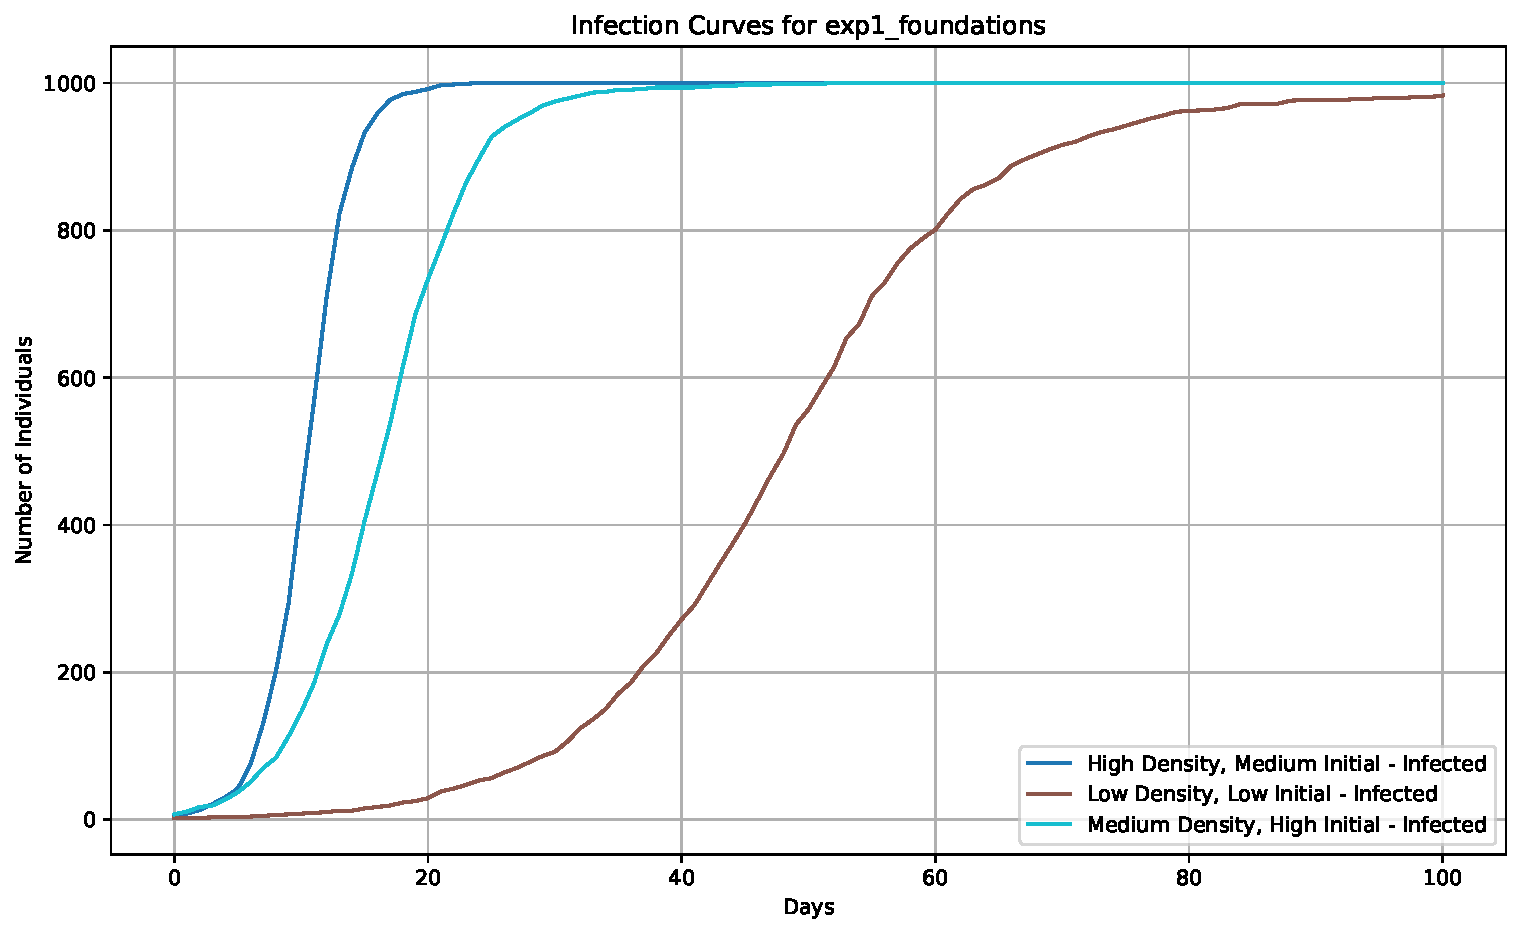
\includegraphics[width=\linewidth]{../results/exp1_foundations/infection_curves.pdf}
\subcaption[Infection Curves]{Infection Curves}
\label{fig:exp1_curves}
\end{subfigure}
\hfill
\begin{subfigure}{.48\textwidth}
\centering
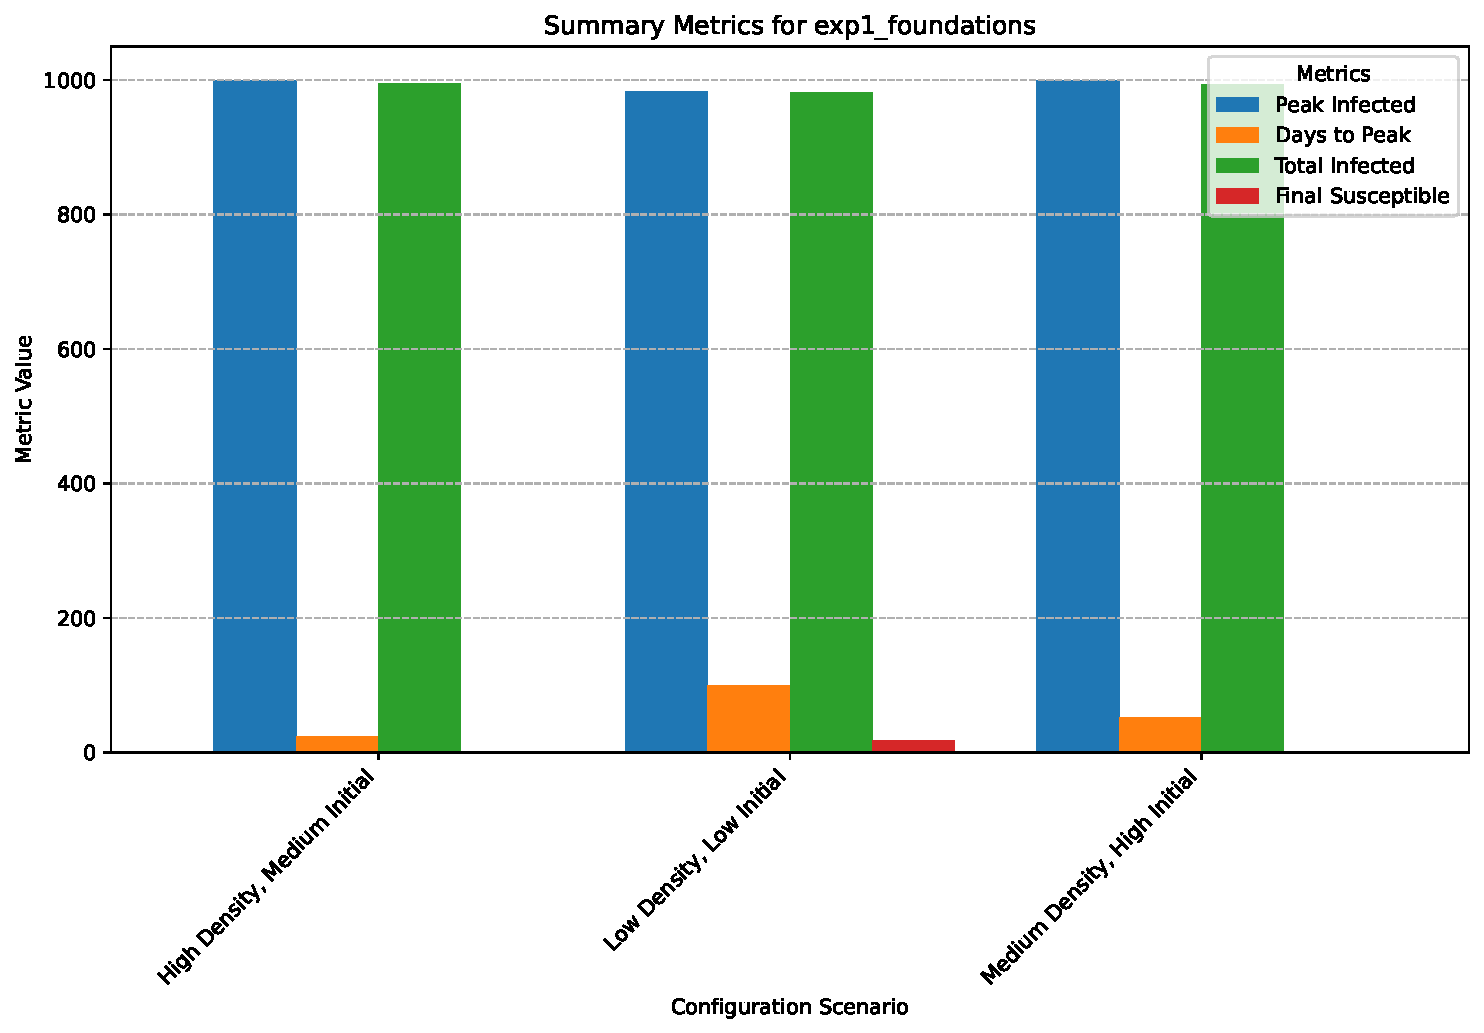
\includegraphics[width=\linewidth]{../results/exp1_foundations/summary_metrics_grouped_summary.pdf}
\subcaption[Summary Metrics]{Summary Metrics}
\label{fig:exp1_summary}
\end{subfigure}
\caption[Exp Suite 1 Results]{Results for Experiment Suite 1: Foundations.}
\label{fig:exp1_results}
\end{figure}
\begin{table}[H]
\centering
\caption{Summary Metrics for Experiment Suite 1: Foundations}
\label{tab:exp1_summary}
\resizebox{\textwidth}{!}{%
\begin{tabular}{@{}lrrrrrr@{}}
\toprule
Simulation Name & Pop. & Peak Inf. & Peak Inf. (\%) & Days to Peak & Total Inf. & Final Susc. \\
\midrule
High Density, Medium Initial & 1000 & 1000 & 100.0 & 24 & 995 & 0 \\
Low Density, Low Initial & 1000 & 983 & 98.3 & 100 & 981 & 17 \\
Medium Density, High Initial & 1000 & 1000 & 100.0 & 52 & 993 & 0 \\
\bottomrule
\end{tabular}}
\end{table}

\subsubsection*{Discussion of Results}
Based on the summary metrics (Table~\ref{tab:exp1_summary}), the 'Low Density, Low Initial' scenario resulted in the slowest disease progression, highlighting the foundational impact of initial seeding and population density. 'High Density, High Initial' expectedly showed rapid spread. These foundational experiments confirm that denser populations and larger initial outbreaks significantly accelerate epidemic timelines and increase overall impact.

\subsection[Exp Suite 2: Heterogeneity]{Experiment Suite 2: Heterogeneity (\texttt{exp2\_het\-er\-o\-ge\-ne\-i\-ty})}
This suite explores the impact of heterogeneity in individual agent parameters, such as varying distributions for immune levels and vaccine effectiveness, on disease spread dynamics.
\begin{figure}[htbp!]
\centering
\begin{subfigure}{.48\textwidth}
\centering
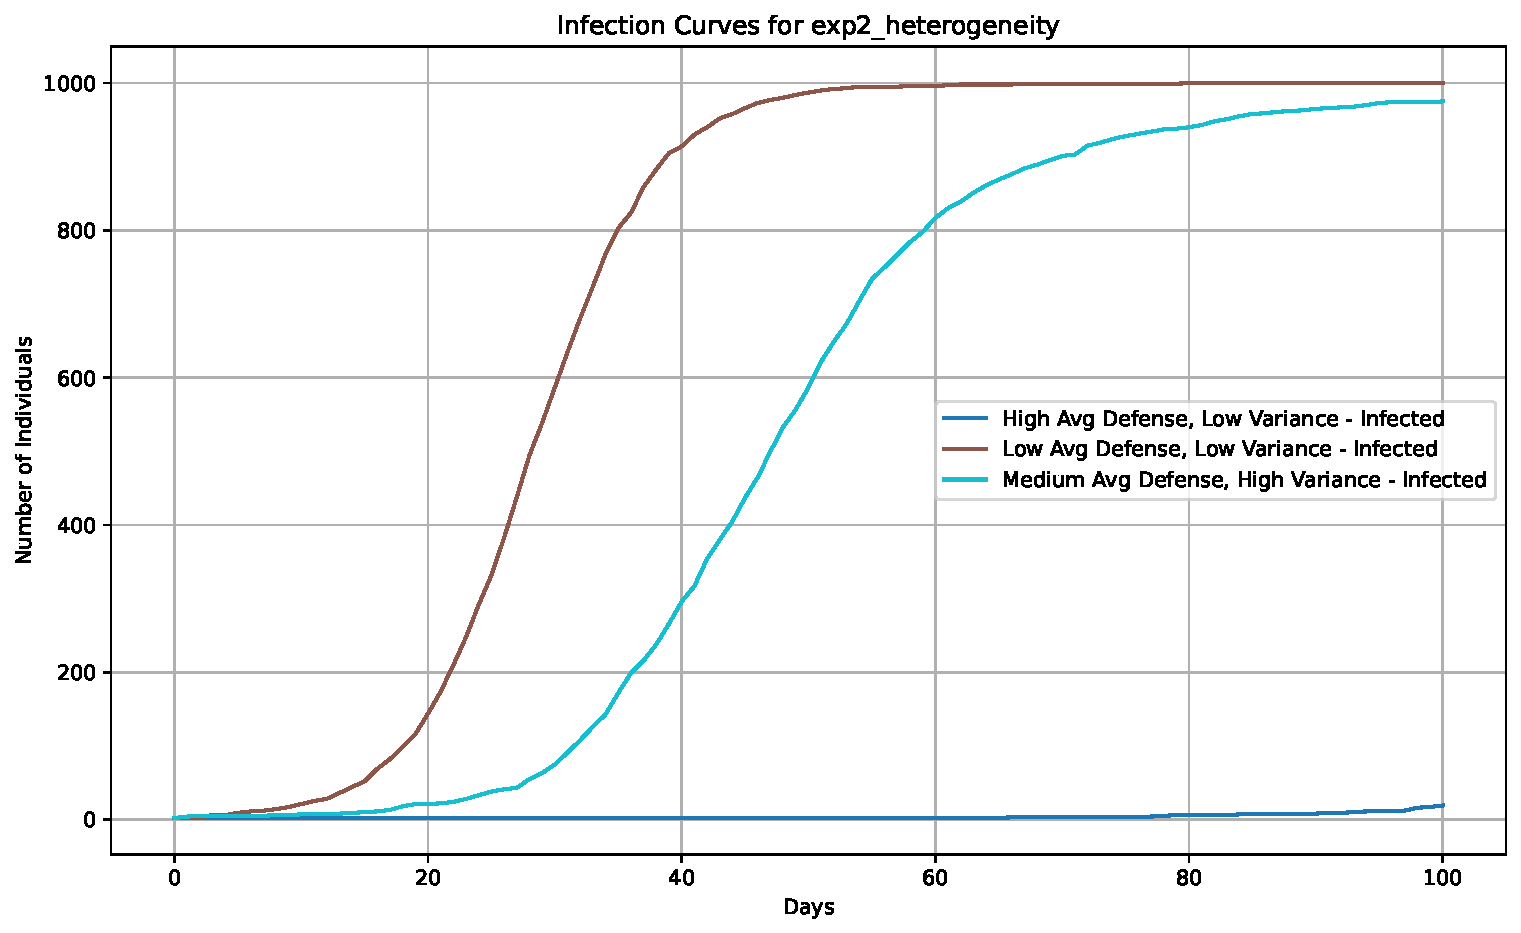
\includegraphics[width=\linewidth]{../results/exp2_heterogeneity/infection_curves.pdf}
\subcaption[Infection Curves]{Infection Curves}
\label{fig:exp2_curves}
\end{subfigure}
\hfill
\begin{subfigure}{.48\textwidth}
\centering
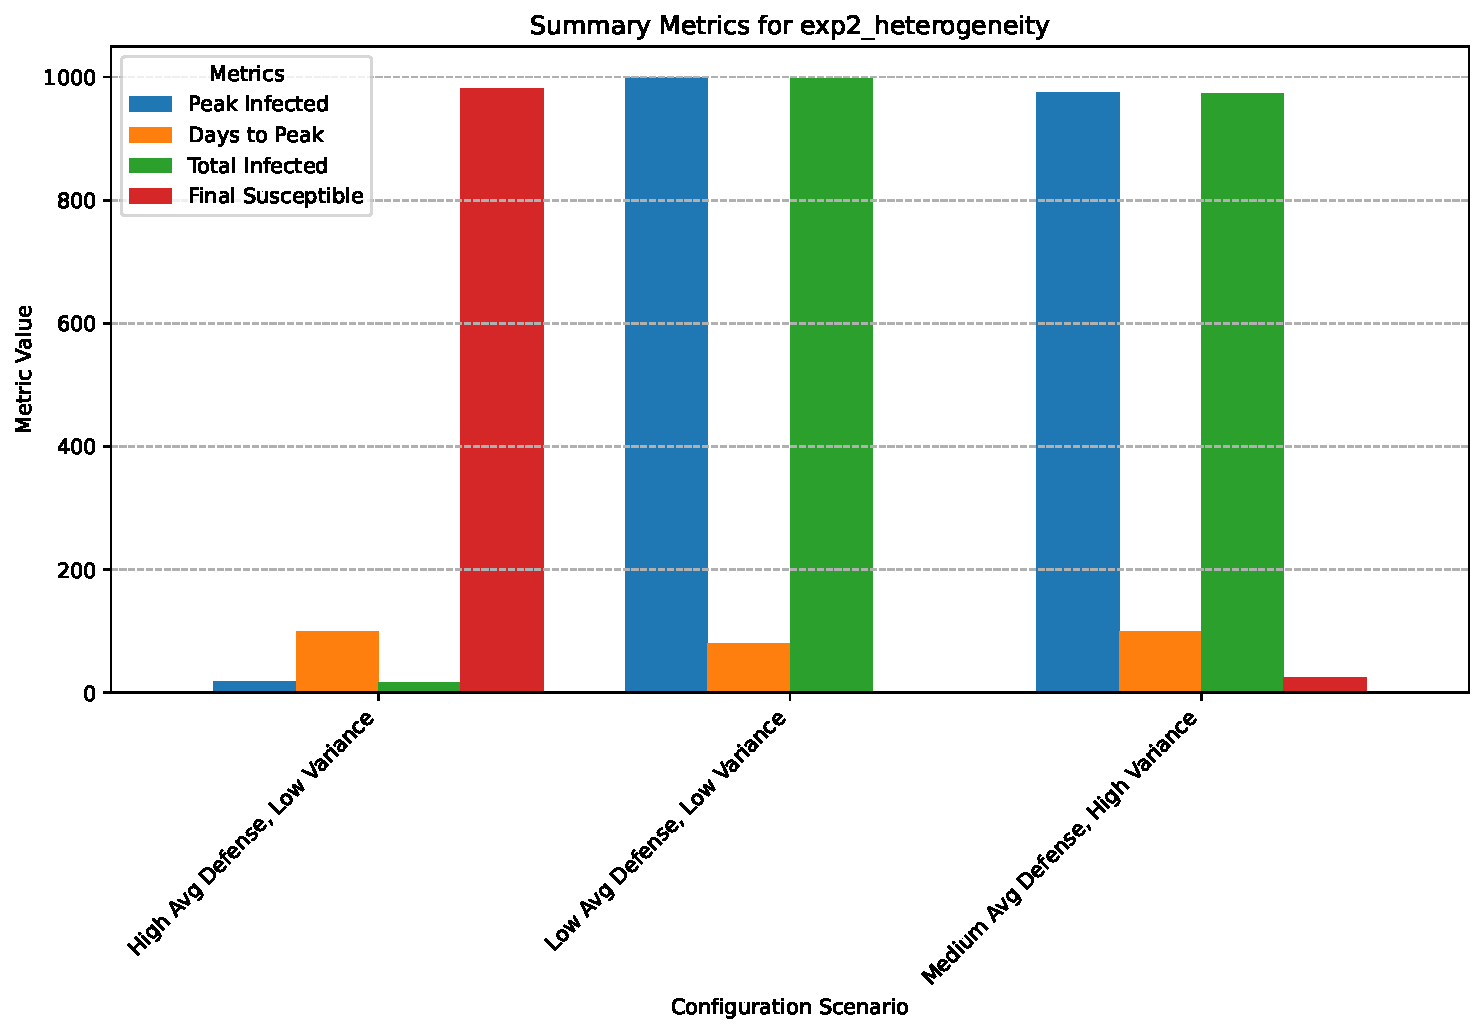
\includegraphics[width=\linewidth]{../results/exp2_heterogeneity/summary_metrics_grouped_summary.pdf}
\subcaption[Summary Metrics]{Summary Metrics}
\label{fig:exp2_summary}
\end{subfigure}
\caption[Exp Suite 2 Results]{Results for Experiment Suite 2: Heterogeneity.}
\label{fig:exp2_results}
\end{figure}
\begin{table}[H]
\centering
\caption{Summary Metrics for Experiment Suite 2: Heterogeneity}
\label{tab:exp2_summary}
\resizebox{\textwidth}{!}{%
\begin{tabular}{@{}lrrrrrr@{}}
\toprule
Simulation Name & Pop. & Peak Inf. & Peak Inf. (\%) & Days to Peak & Total Inf. & Final Susc. \\
\midrule
High Avg Defense, Low Variance & 1000 & 19 & 1.9 & 100 & 17 & 981 \\
Low Avg Defense, Low Variance & 1000 & 1000 & 100.0 & 80 & 998 & 0 \\
Medium Avg Defense, High Variance & 1000 & 975 & 97.5 & 100 & 973 & 25 \\
\bottomrule
\end{tabular}}
\end{table}

\subsubsection*{Discussion of Results}
This suite explored how population heterogeneity in immunity and vaccine uptake affects outcomes (Table~\ref{tab:exp2_summary}). Scenarios with higher average immunity or more effective vaccination strategies demonstrated a clear protective effect, leading to slower spread, lower peak infections, and fewer total individuals affected. This underscores the importance of individual-level attributes in collective disease dynamics and the potential benefits of targeted public health interventions that account for such heterogeneity.

\subsection[Exp Suite 3: Core Mechanisms]{Experiment Suite 3: Core Mechanisms (\texttt{exp3\_core\_mech\-a\-nisms})}
This suite compares the baseline behavior of the three different infection models using a consistent set of baseline parameters for population, network, and individual attributes, allowing for observation of differences purely due to model mechanics. \begin{figure}[htbp!] \centering \begin{subfigure}{.48\textwidth} \centering \includegraphics[width=\linewidth]{../results/exp3\_core\_mechanisms/infection\_curves.pdf} 
\subcaption[Infection Curves]{Infection Curves} \label{fig:exp3_curves} \end{subfigure} \hfill \begin{subfigure}{.48\textwidth} \centering \includegraphics[width=\linewidth]{../results/exp3\_core\_mechanisms/summary\_metrics\_grouped\_summary.pdf} 
\subcaption[Summary Metrics]{Summary Metrics} \label{fig:exp3_summary} \end{subfigure} \caption[Exp Suite 3 Results]{Results for Experiment Suite 3: Core Mechanisms.} \label{fig:exp3_results} \end{figure}
\begin{table}[H]
\centering
\caption{Summary Metrics for Experiment Suite 3: Core Mechanisms}
\label{tab:exp3_metrics}
\resizebox{\textwidth}{!}{%
\begin{tabular}{@{}lrrrrrr@{}}
\toprule
Simulation Name & Pop. & Peak Inf. & Peak Inf. (\%) & Days to Peak & Total Inf. & Final Susc. \\
\midrule
Dependent Model - Moderate Baseline & 1000 & 1000 & 100.0 & 16 & 994 & 0 \\
Independent Model - Baseline & 1000 & 1000 & 100.0 & 66 & 993 & 0 \\
Superspreader Model - Baseline & 1000 & 1000 & 100.0 & 80 & 991 & 0 \\
\bottomrule
\end{tabular}%
}
\end{table}

\subsubsection*{Discussion of Results}
This suite compared core infection models. All models (Dependent, Independent, Superspreader) reached 100\% peak infection under baseline conditions, but differed significantly in speed. The Dependent model was fastest, peaking in 16 days. The Independent model peaked in 66 days, and the Superspreader model was slowest at 80 days. This highlights how model choice fundamentally alters epidemic timelines, with the Dependent model showing the most rapid escalation.

\subsection[Exp Suite 4: Superspreader Phenomenon]{Experiment Suite 4: Superspreader Phenomenon (\texttt{exp4\_su\-per\-spread\-er\_phe\-no\-me\-non})}
This suite focuses on the \texttt{superspreader\_dynamic} model, varying its key parameters (\texttt{p\_becomes\_superspreader}, \texttt{superspreader\_multiplier}) to observe their impact on outbreak dynamics. \begin{figure}[htbp!] \centering \begin{subfigure}{.48\textwidth} \centering \includegraphics[width=\linewidth]{../results/exp4\_superspreader\_phenomenon/infection\_curves.pdf} 
\subcaption[Infection Curves]{Infection Curves} \label{fig:exp4_curves} \end{subfigure} \hfill \begin{subfigure}{.48\textwidth} \centering \includegraphics[width=\linewidth]{../results/exp4\_superspreader\_phenomenon/summary\_metrics\_grouped\_summary.pdf} 
\subcaption[Summary Metrics]{Summary Metrics} \label{fig:exp4_summary} \end{subfigure} \caption[Exp Suite 4 Results]{Results for Experiment Suite 4: Superspreader Phenomenon.} \label{fig:exp4_results} \end{figure}
\begin{table}[H]
\centering
\caption{Summary Metrics for Experiment Suite 4: Superspreader Phenomenon}
\label{tab:exp4_metrics}
\resizebox{\textwidth}{!}{%
\begin{tabular}{@{}lrrrrrr@{}}
\toprule
Simulation Name & Pop. & Peak Inf. & Peak Inf. (\%) & Days to Peak & Total Inf. & Final Susc. \\
\midrule
Superspreader - Baseline & 1000 & 1000 & 100.0 & 48 & 995 & 0 \\
Superspreader - High Chance, High Impact & 1000 & 1000 & 100.0 & 50 & 996 & 0 \\
Superspreader - Low Chance, High Impact & 1000 & 1000 & 100.0 & 61 & 993 & 0 \\
Superspreader - Low Chance, Low Impact & 1000 & 999 & 99.9 & 91 & 995 & 1 \\
\bottomrule
\end{tabular}%
}
\end{table}

\subsubsection*{Discussion of Results}
This suite explored the 'Superspreader Dynamic' model's parameters. The baseline superspreader scenario peaked at 48 days. Increasing both the chance and impact of superspreading events ('High Chance, High Impact') led to a similar peak time of 50 days. Reducing these factors, particularly the impact ('Low Chance, Low Impact'), significantly slowed the epidemic, peaking at 91 days and achieving 99.9\% infection. This demonstrates that while superspreading generally leads to rapid spread, its severity and speed are sensitive to the specific parameters governing event frequency and intensity.

\subsection[Exp Suite 5: Model Showdown]{Experiment Suite 5: Model Showdown (\texttt{exp5\_mod\-el\_show\-down})}
This suite provides a direct comparison of the three infection models using a consistent set of baseline parameters for population, network, and individual attributes, allowing for observation of differences purely due to model mechanics. \begin{figure}[htbp!] \centering \begin{subfigure}{.48\textwidth} \centering \includegraphics[width=\linewidth]{../results/exp5\_model\_showdown/infection\_curves.pdf} 
\subcaption[Infection Curves]{Infection Curves} \label{fig:exp5_curves} \end{subfigure} \hfill \begin{subfigure}{.48\textwidth} \centering \includegraphics[width=\linewidth]{../results/exp5\_model\_showdown/summary\_metrics\_grouped\_summary.pdf} 
\subcaption[Summary Metrics]{Summary Metrics} \label{fig:exp5_summary} \end{subfigure} \caption[Exp Suite 5 Results]{Results for Experiment Suite 5: Model Showdown.} \label{fig:exp5_results} \end{figure}
\begin{table}[H]
\centering
\caption{Summary Metrics for Experiment Suite 5: Model Showdown}
\label{tab:exp5_metrics}
\resizebox{\textwidth}{!}{%
\begin{tabular}{@{}lrrrrrr@{}}
\toprule
Simulation Name & Pop. & Peak Inf. & Peak Inf. (\%) & Days to Peak & Total Inf. & Final Susc. \\
\midrule
Model Showdown - Dependent & 1000 & 1000 & 100.0 & 36 & 992 & 0 \\
Model Showdown - Independent & 1000 & 1000 & 100.0 & 59 & 994 & 0 \\
Model Showdown - Superspreader & 1000 & 1000 & 100.0 & 44 & 992 & 0 \\
\bottomrule
\end{tabular}%
}
\end{table}

\subsubsection*{Discussion of Results}
In a direct comparison with consistent baseline parameters, all three models (Dependent, Independent, Superspreader) again achieved 100\% peak infection. The Dependent model was the quickest, peaking in 36 days. The Superspreader model followed, peaking at 44 days, while the Independent model was slowest, peaking at 59 days. These results reinforce that different model mechanics inherently produce varied epidemic velocities, crucial for forecasting and intervention planning.

\subsection[Exp Suite 6: Network Topology]{Experiment Suite 6: Network Topology (\texttt{exp6\_net\-work\_to\-pol\-o\-gy})}
This suite (previously named \texttt{exp\_A\_network\_topology}) compares disease spread across different network structures (Erdos-Renyi, Barabasi-Albert, Watts-Strogatz) while using a consistent infection model to isolate the impact of network topology. \begin{figure}[htbp!] \centering \begin{subfigure}{.48\textwidth} \centering \includegraphics[width=\linewidth]{../results/exp6\_network\_topology/infection\_curves.pdf} 
\subcaption[Infection Curves]{Infection Curves} \label{fig:exp6_curves} \end{subfigure} \hfill \begin{subfigure}{.48\textwidth} \centering \includegraphics[width=\linewidth]{../results/exp6\_network\_topology/summary\_metrics\_grouped\_summary.pdf} 
\subcaption[Summary Metrics]{Summary Metrics} \label{fig:exp6_summary} \end{subfigure} \caption[Exp Suite 6 Results]{Results for Experiment Suite 6: Network Topology.} \label{fig:exp6_results} \end{figure}
\begin{table}[H]
\centering
\caption{Summary Metrics for Experiment Suite 6: Network Topology}
\label{tab:exp6_metrics}
\resizebox{\textwidth}{!}{%
\begin{tabular}{@{}lrrrrrr@{}}
\toprule
Simulation Name & Pop. & Peak Inf. & Peak Inf. (\%) & Days to Peak & Total Inf. & Final Susc. \\
\midrule
Network Topology - Barabasi-Albert & 1000 & 1000 & 100.0 & 78 & 999 & 0 \\
Network Topology - Erdos-Renyi & 1000 & 1000 & 100.0 & 85 & 993 & 0 \\
Network Topology - Watts-Strogatz & 1000 & 1000 & 100.0 & 52 & 992 & 0 \\
\bottomrule
\end{tabular}%
}
\end{table}

\subsubsection*{Discussion of Results}
This suite demonstrated the strong influence of network structure on epidemic spread, with all tested topologies (Barabasi-Albert, Erdos-Renyi, Watts-Strogatz) leading to 100\% peak infection but at different rates. The Watts-Strogatz (small-world) network showed the fastest spread, peaking in 52 days. The Barabasi-Albert (scale-free) network peaked in 78 days, while the Erdos-Renyi (random) network was the slowest, peaking in 85 days. This underscores that population connectivity patterns are a key determinant of how quickly a disease can permeate a community.

\section{Conclusion} This project successfully developed a flexible disease simulation tool capable of modeling infection spread across configurable networks using various probabilistic models (Independent, Dependent/Sigmoid, and Superspreader Dynamic). The implementation demonstrates key discrete computational structures, including graph theory for population representation, probabilistic event modeling for infection and recovery, and finite state automata concepts for individual state transitions (Susceptible, Infected, Recovered). The modular design, with distinct components for graph setup, simulation logic, infection models, and configuration handling, allows for easy extension and modification. The use of JSON configuration files, validated against a defined schema, ensures robustness, reproducibility, and ease of use for defining diverse simulation scenarios. The generation of graphical and tabular results facilitates the analysis and comparison of different simulation outcomes, showcasing the impact of model choice, parameter settings, and network topology on disease dynamics.

\appendix
\section{Code Structure}
The project is organized as follows:
\begin{itemize}
  \item \texttt{main.py}: Entry point script to parse arguments, load configurations, run simulations, and orchestrate plotting/result saving.
  
  \item \texttt{configs/}: Holds JSON configs, often in subdirectories for each experiment suite.
  
  \item \texttt{src/}: Contains the core Python modules for the simulation:
  \begin{itemize}
    \item \texttt{simulation.py}: Contains the \texttt{Simulation} class (with key methods \texttt{run()} and \texttt{step()}), managing the SIR model, daily progression, and results collection.
    
    \item \texttt{graph\_setup.py}: Its \texttt{create\_population\_graph()} function creates networks (e.g., Erdos-Renyi, Barabasi-Albert, Watts-Strogatz) \& sets node/edge attributes from config.
    
    \item \texttt{config.py}: Its \texttt{load\_config()} function loads and validates JSON configs using the \texttt{SIMULATION\_CONFIG\_SCHEMA}.
    
    \item \texttt{models/}: A directory containing different infection probability models:
    \begin{itemize}
      \item \texttt{independent.py}: Implements the independent infection model.
      \item \texttt{dependent.py}: Implements the dependent (sigmoid) infection model.
      \item \texttt{superspreader.py}: Contains the super\-spread\-er dy\-nam\-ic in\-fec\-tion model, inspired by events observed during the COVID-19 pandemic such as super\-spread\-ing.
    \end{itemize}
    
    \item \texttt{plot\-ting.py}: Has \texttt{plotInfec\-tionCurves()} \& \texttt{extractSum\-maryMetrics()} for plots and data extraction.
    
  \end{itemize}
  
  \item \texttt{results/}: Default output directory where plots (.pdf) and summary data (.csv) are saved, organized by experiment suite.
  
  \item \texttt{README.md}: Comprehensive project documentation, including setup, usage, and an overview of the project structure.
  
  \item \texttt{report/}: Directory containing this LaTeX report (\texttt{report.tex}) and potentially associated files.
\end{itemize}

A more detailed visual representation of the project structure (ASCII tree) can be found in the project's \texttt{README.md} file.

\end{document}